\documentclass[a4paper, 14pt]{extarticle}
\UseRawInputEncoding

% Поля
%--------------------------------------
\usepackage{geometry}
\geometry{a4paper,tmargin=2cm,bmargin=2cm,lmargin=3cm,rmargin=1cm}
%--------------------------------------


%Russian-specific packages
%--------------------------------------
\usepackage[T2A]{fontenc}
\usepackage[utf8]{inputenc} 
\usepackage[english, main=russian]{babel}
%--------------------------------------

\usepackage{textcomp}

% Красная строка
%--------------------------------------
\usepackage{indentfirst}               
%--------------------------------------             


%Graphics
%--------------------------------------
\usepackage{graphicx}
\graphicspath{ {./images/} }
\usepackage{wrapfig}
%--------------------------------------

% Полуторный интервал
%--------------------------------------
\linespread{1.3}                    
%--------------------------------------

%Выравнивание и переносы
%--------------------------------------
% Избавляемся от переполнений
\sloppy
% Запрещаем разрыв страницы после первой строки абзаца
\clubpenalty=10000
% Запрещаем разрыв страницы после последней строки абзаца
\widowpenalty=10000
%--------------------------------------

%Списки
\usepackage{enumitem}

%Подписи
\usepackage{caption} 

%Гиперссылки
\usepackage{hyperref}

\hypersetup {
	unicode=true
}

%Рисунки
%--------------------------------------
\DeclareCaptionLabelSeparator*{emdash}{~--- }
\captionsetup[figure]{labelsep=emdash,font=onehalfspacing,position=bottom}
%--------------------------------------

\usepackage{tempora}

%Листинги
%--------------------------------------
\usepackage{listings}
\lstset{
  basicstyle=\ttfamily\footnotesize, 
  %basicstyle=\footnotesize\AnkaCoder,        % the size of the fonts that are used for the code
  breakatwhitespace=false,         % sets if automatic breaks shoulbd only happen at whitespace
  breaklines=true,                 % sets automatic line breaking
  captionpos=t,                    % sets the caption-position to bottom
  inputencoding=utf8,
  frame=single,                    % adds a frame around the code
  keepspaces=true,                 % keeps spaces in text, useful for keeping indentation of code (possibly needs columns=flexible)
  keywordstyle=\bf,       % keyword style
  numbers=left,                    % where to put the line-numbers; possible values are (none, left, right)
  numbersep=5pt,                   % how far the line-numbers are from the code
  xleftmargin=25pt,
  xrightmargin=25pt,
  showspaces=false,                % show spaces everywhere adding particular underscores; it overrides 'showstringspaces'
  showstringspaces=false,          % underline spaces within strings only
  showtabs=false,                  % show tabs within strings adding particular underscores
  stepnumber=1,                    % the step between two line-numbers. If it's 1, each line will be numbered
  tabsize=2,                       % sets default tabsize to 8 spaces
  title=\lstname                   % show the filename of files included with \lstinputlisting; also try caption instead of title
}
%--------------------------------------

%%% Математические пакеты %%%
%--------------------------------------
\usepackage{amsthm,amsfonts,amsmath,amssymb,amscd}  % Математические дополнения от AMS
\usepackage{mathtools}                              % Добавляет окружение multlined
\usepackage[perpage]{footmisc}
%--------------------------------------

%--------------------------------------
%			НАЧАЛО ДОКУМЕНТА
%--------------------------------------

\begin{document}

%--------------------------------------
%			ТИТУЛЬНЫЙ ЛИСТ
%--------------------------------------
\begin{titlepage}
\thispagestyle{empty}
\newpage


%Шапка титульного листа
%--------------------------------------
\vspace*{-60pt}
\hspace{-65pt}
\begin{minipage}{0.3\textwidth}
\hspace*{-20pt}\centering

\includegraphics[width=\textwidth]{emblem}
\end{minipage}
\begin{minipage}{0.67\textwidth}\small \textbf{
\vspace*{-0.7ex}
\hspace*{-6pt}\centerline{Министерство науки и высшего образования Российской Федерации}
\vspace*{-0.7ex}
\centerline{Федеральное государственное бюджетное образовательное учреждение }
\vspace*{-0.7ex}
\centerline{высшего образования}
\vspace*{-0.7ex}
\centerline{<<Московский государственный технический университет}
\vspace*{-0.7ex}
\centerline{имени Н.Э. Баумана}
\vspace*{-0.7ex}
\centerline{(национальный исследовательский университет)>>}
\vspace*{-0.7ex}
\centerline{(МГТУ им. Н.Э. Баумана)}}
\end{minipage}
%--------------------------------------

%Полосы
%--------------------------------------
\vspace{-25pt}
\hspace{-35pt}\rule{\textwidth}{2.3pt}

\vspace*{-20.3pt}
\hspace{-35pt}\rule{\textwidth}{0.4pt}
%--------------------------------------

\vspace{1.5ex}
\hspace{-35pt} \noindent \small ФАКУЛЬТЕТ\hspace{80pt} <<Информатика и системы управления>>

\vspace*{-16pt}
\hspace{47pt}\rule{0.83\textwidth}{0.4pt}

\vspace{0.5ex}
\hspace{-35pt} \noindent \small КАФЕДРА\hspace{50pt} <<Теоретическая информатика и компьютерные технологии>>

\vspace*{-16pt}
\hspace{30pt}\rule{0.866\textwidth}{0.4pt}
  
\vspace{11em}

\begin{center}
\Large {\bf Лабораторная работа № 1} \\ 
\large {\bf по курсу <<Алгоритмы компьютерной графики>>} \\
% \large <<Разработка SMTP-клиента и приложения почтовой рассылки>> 
\end{center}\normalsize

\vspace{8em}


\begin{flushright}
  {Студент группы ИУ9-41Б Горбунов А. Д. \hspace*{15pt}\\ 
  \vspace{2ex}
  Преподаватель Целкович П. А.\hspace*{15pt}}
\end{flushright}

\bigskip

\vfill
 

\begin{center}
\textsl{Москва 2024}
\end{center}
\end{titlepage}
%--------------------------------------
%		КОНЕЦ ТИТУЛЬНОГО ЛИСТА
%--------------------------------------

\renewcommand{\ttdefault}{pcr}

\setlength{\tabcolsep}{3pt}
\newpage
\setcounter{page}{2}

\section{Задание}\label{Sect::task}
    Используя OpenGL создать: многоугольник у которого 4 или больше углов и сделать взаимодействие с ним

    
\section{Результаты}\label{Sect::res}

Исходный код программы представлен в листинге~\ref{lst:code1}, ~\ref{lst:code2}

\begin{figure}[!htb]
\begin{lstlisting}[language={c++},caption={main.cpp},label={lst:code1}]
#include <GL/gl.h>
#include <GLFW/glfw3.h>
#include <iostream>

float degree_y = 0.0;
float degree_x = 0.0;
float move_y = 0.0;
float move_x = 0.0;

void key(GLFWwindow *window, int key, int scancode, int action, int mods)
{
    if (action == GLFW_PRESS)
    {
        if (key == GLFW_KEY_ESCAPE)    { glfwSetWindowShouldClose(window, GL_TRUE);   }
        else if (key == GLFW_KEY_UP)   { degree_y += 0.2;  }
        else if (key == GLFW_KEY_DOWN) { degree_y -= 0.2;  }
        else if (key == GLFW_KEY_LEFT) { degree_x += 0.2;  }
        else if (key == GLFW_KEY_RIGHT){ degree_x -= 0.2;  }
        else if (key == GLFW_KEY_D)    { move_x += 0.2;    }
        else if (key == GLFW_KEY_A)    { move_x -= 0.2;    }
        else if (key == GLFW_KEY_W)    { move_y += 0.2;    }
        else if (key == GLFW_KEY_S)    { move_y -= 0.2;    }
    }
}
\end{lstlisting}
\end{figure}

\begin{figure}[!htb]
\begin{lstlisting}[language={c++},caption={main.cpp(продолжение)},label={lst:code2}]
void display(GLFWwindow *window)
{
    glClear(GL_COLOR_BUFFER_BIT);
    glMatrixMode(GL_PROJECTION);
    glLoadIdentity();
    glMatrixMode(GL_MODELVIEW);
    glLoadIdentity();
    glRotatef(degree_y * 50.f, 1.f, 0.f, 0.f);
    glRotatef(degree_x * 50.f, 0.f, 0.f, 1.f);
    glBegin(GL_POLYGON);
    glColor3f(1, 0, 0);
    glVertex2f(move_x+0.25, move_y+0);
    glColor3f(0, 1, 0);
    glVertex2f(move_x+0.25, move_y+0.5);
    glColor3f(0, 0, 1);
    glVertex2f(move_x+(-0.25), move_y+0.5);
    glColor3f(0, 1, 1);
    glVertex2f(move_x+(-0.25), move_y+0);
    glEnd();
    glPopMatrix();
}
int main(int argc, char const *argv[])
{
    if (!glfwInit())
        exit(1);
    glfwWindowHint (GLFW_RESIZABLE, 1);
    GLFWwindow *window = glfwCreateWindow(1920, 1080, "Lab 1", glfwGetPrimaryMonitor(), NULL);
    if (window == NULL)
    {
        glfwTerminate();
        exit(1);
    }    
    glfwMakeContextCurrent(window);
    glfwSwapInterval(1);
    glfwSetKeyCallback(window, key);
    while (!glfwWindowShouldClose(window))
    {
        display(window);
        glfwSwapBuffers(window);
        glfwPollEvents();
    }
    glfwDestroyWindow(window);
    glfwTerminate();
    return 0;
}
\end{lstlisting}
\end{figure}

\begin{figure}[!htb]
Результат запуска представлен на рисунке ~\ref{fig:picture_1.png}, ~\ref{fig:picture_2.png}
\end{figure}

\begin{figure}[!htb]
	\centering
	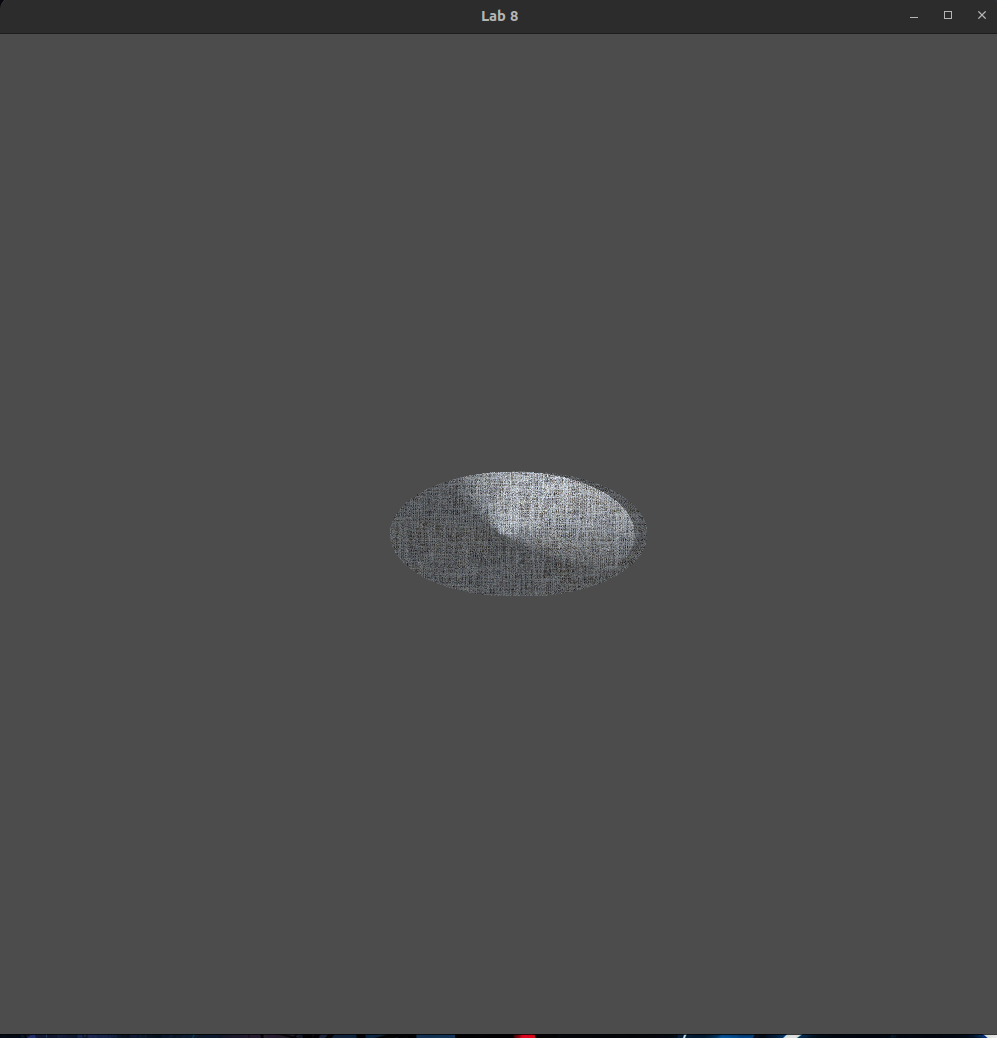
\includegraphics[width=0.8\textwidth]{picture_1.png}
\caption{Без воздействия}
\label{fig:picture_1.png}
\end{figure}

\begin{figure}[!htb]
	\centering
	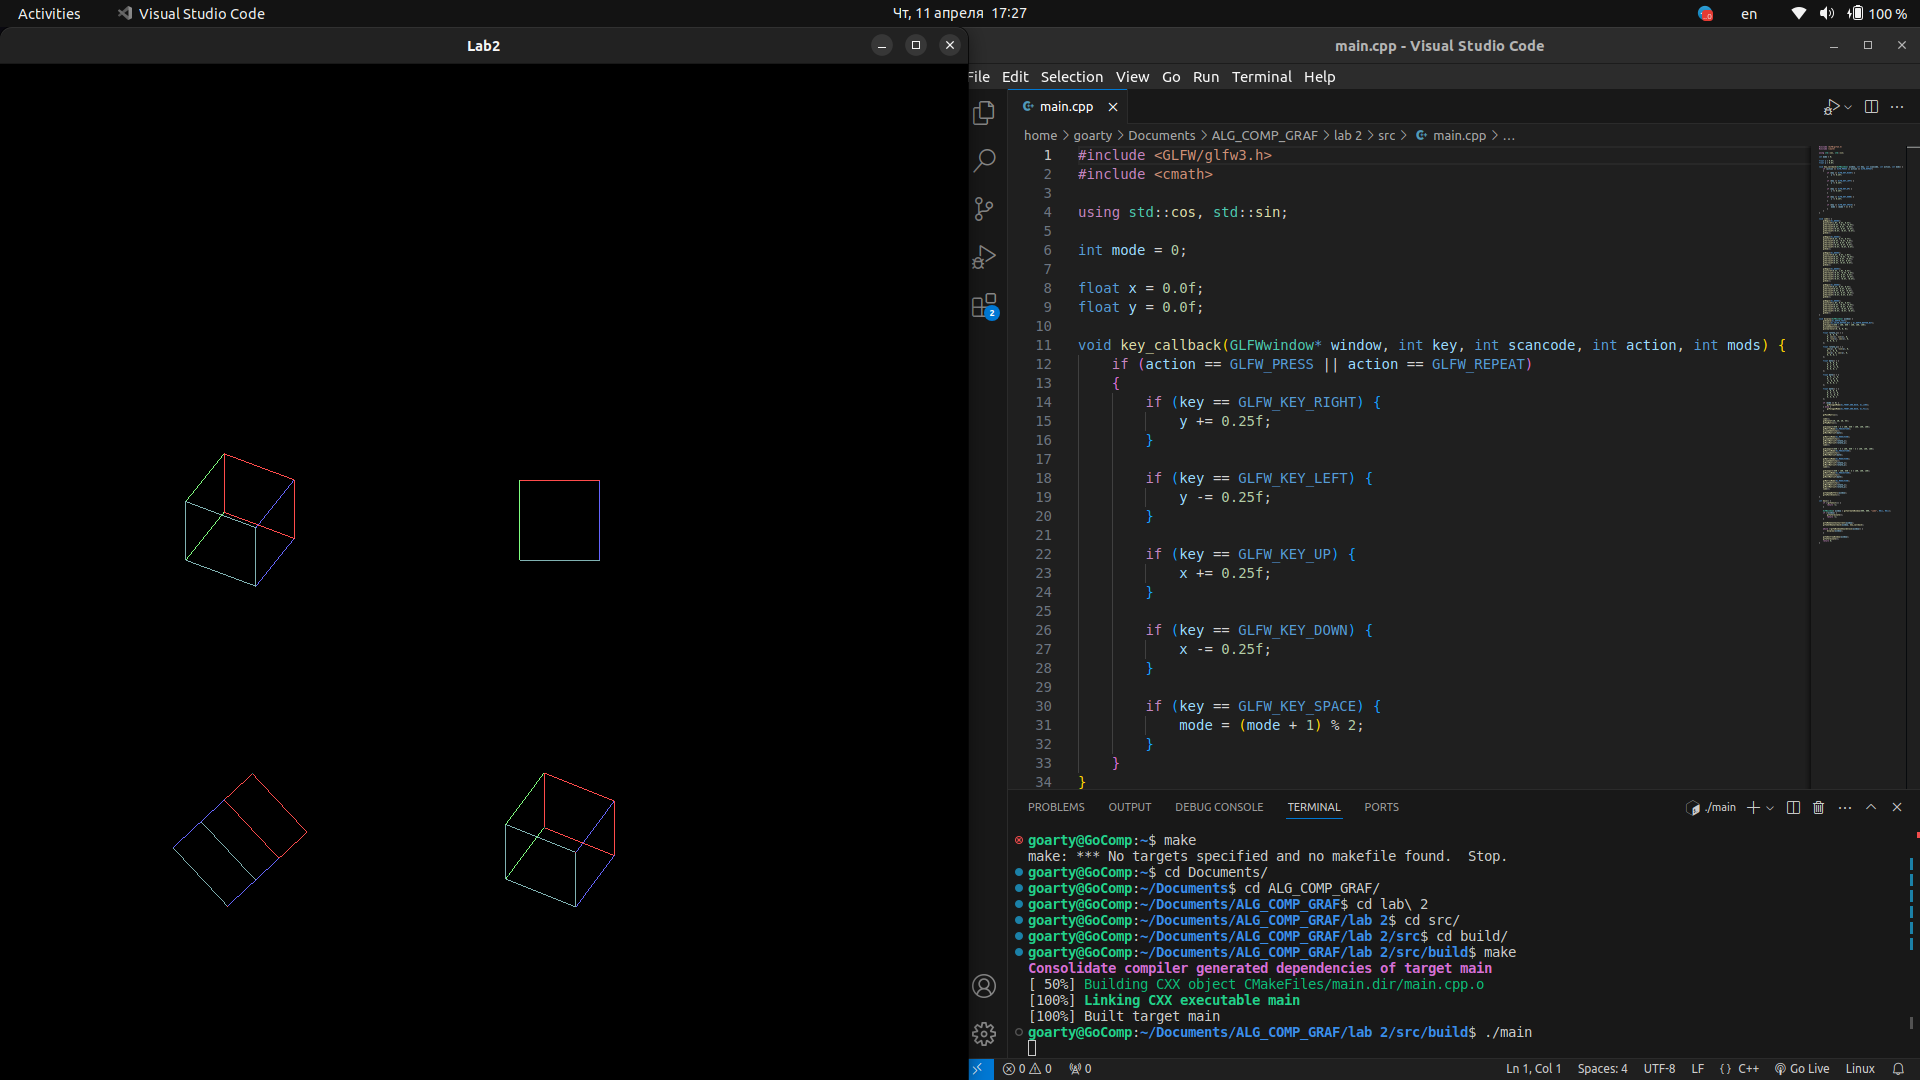
\includegraphics[width=0.8\textwidth]{picture_2.png}
\caption{Со смещением и поворотом}
\label{fig:picture_2.png}
\end{figure}

\end{document}
